\documentclass[conference]{IEEEtran}
\usepackage{cite}
\usepackage{amsmath,amssymb,amsfonts}
\usepackage{algorithmic}
\usepackage{graphicx}
\usepackage{textcomp}
\usepackage{xcolor}
\usepackage{booktabs}
\usepackage{multirow}
\usepackage{array}
\usepackage{tikz}
\usetikzlibrary{shapes,arrows,positioning,calc,fit,backgrounds,decorations.pathreplacing}
\usepackage{pgfplots}
\pgfplotsset{compat=1.17}
\usepackage{hyperref}
\usepackage{url}
\usepackage{stfloats}

\def\BibTeX{{\rm B\kern-.05em{\sc i\kern-.025em b}\kern-.08em
    T\kern-.1667em\lower.7ex\hbox{E}\kern-.125emX}}

\begin{document}

\title{Temporal-Linguistic Adaptive Streaming for Continuous Sign Language Translation}

\author{
\IEEEauthorblockN{Arshia Kermani, Habib Irani, Vangelis Metsis}
\IEEEauthorblockA{
\textit{Department of Computer Science}\\
\textit{Texas State University}\\
San Marcos, TX, USA\\
\{arshia.kermani,habibirani,vmetsis\}@txstate.edu
}
}

\maketitle

\begin{abstract}
Real-time sign language translation must generate text incrementally as signs arrive, yet existing streaming policies treat glosses as a flat token sequence and discard the temporal rhythm of signing. Inter-gloss pauses reliably mark sentence boundaries in continuous discourse, but policies such as Wait-k cause arbitrary cross-boundary fragmentation. We propose \textbf{Temporal-Linguistic Adaptive Streaming} (TLAS), which fuses a Temporal Pause Detector (TPD, tracking inter-gloss interval statistics via an exponential moving average) and a Linguistic Readiness Estimator (LRE, a trained neural head on a frozen T5 encoder) through an Adaptive Fusion Gate (AFG). A proactive timeout fires \emph{before} the next gloss arrives when the inter-gloss gap exceeds $2.5\times$ the running average, producing clean sentence segmentation without oracle boundary information. We also contribute a synthetic discourse dataset of 1,400 ASL discourse groups with LLM-generated per-gloss timestamps and introduce a continuous-stream evaluation paradigm requiring autonomous boundary detection from an unbroken gloss stream. Under such conditions, TLAS significantly outperforms current heuristic baselines, such as Wait-k, and methods relying solely on linguistic content.
\end{abstract}

\begin{IEEEkeywords}
sign language translation, streaming translation, simultaneous interpretation, temporal pause detection, linguistic readiness estimation, adaptive fusion, discourse segmentation, synthetic dataset
\end{IEEEkeywords}

\section{Introduction}

Approximately 70 million people worldwide rely on sign languages as their primary mode of communication \cite{who2021}. In healthcare triage, legal proceedings, and emergency response, the absence of a real-time interpreter can delay diagnoses, produce inadmissible testimony, or prevent timely access to services. Automated sign language translation systems capable of operating in real time would substantially reduce these barriers; yet the large majority of existing systems require a complete, pre-recorded input before producing any output, making them unsuitable for interactive deployment.

A central challenge in building sign language translation pipelines is the structural mismatch between visual sign production and spoken-language text. American Sign Language (ASL) employs spatial grammar, topic-comment ordering, and non-manual markers that do not correspond one-to-one with English syntax. A direct video-to-text approach must simultaneously solve the recognition problem (mapping continuous visual motion to discrete linguistic units) and the translation problem (mapping one language to another), two high-complexity tasks whose error rates compound. The standard solution is a two-stage pipeline: a vision module converts video frames into a sequence of \emph{glosses}, discrete lexical labels assigned monotonically to individual signs, and a translation model maps the resulting gloss sequence to fluent target text \cite{koller2015continuous,camgoz2018neural}. The monotonic gloss-to-token correspondence makes streaming translation tractable: as each gloss arrives, the system can decide, based on accumulated context, whether to wait for additional signs or commit to generating output. This paper addresses the gloss-to-text stage under real-time, continuous-stream conditions.

Existing streaming policies borrowed from spoken-language simultaneous translation fail to exploit a modality-specific signal that is readily available in the gloss stream: the temporal rhythm of signing. Within a sentence, inter-gloss intervals range from approximately 300 to 650~ms; between sentences, signers pause for 2 to 7~seconds. Wait-k \cite{ma2019stacl} and TransLLaMa \cite{koshkin2024transllama} treat the gloss stream as a flat token sequence and make read/write decisions solely from linguistic content, discarding this temporal information entirely. As a consequence, both policies fragment multi-sentence discourse arbitrarily across boundaries, forcing the translation backend to complete incoherent partial sentences or produce hallucinated continuations. A policy that monitors inter-gloss gap statistics could instead detect sentence boundaries before the next sentence begins, enabling clean segmentation and preserving discourse coherence across translations.

A further obstacle to progress is the absence of publicly available datasets that pair continuous discourse gloss streams with per-gloss arrival timestamps. Without such a benchmark, it is impossible to measure continuous-stream segmentation quality or to study the effect of timestamp degradation (e.g., jitter introduced by a real-time vision module) on translation policies. Existing resources such as ASLG-PC12 \cite{othman2012english} provide isolated sentence pairs without temporal annotations, and sentence-level evaluation conceals the boundary-detection failures that dominate real-world deployment.

In this work, we propose the \textbf{Temporal-Linguistic Adaptive Streaming} (TLAS) policy, which integrates two complementary readiness signals before committing to a translation: (a) the \textbf{Temporal Pause Detector} (TPD), which maintains an exponential moving average of inter-gloss gaps and emits a pause score $s_t \in [0,1]$ that rises during inter-sentence silences, and (b) the \textbf{Linguistic Readiness Estimator} (LRE), a lightweight neural head on a frozen T5 encoder~\cite{raffel2020exploring} that scores the grammatical completeness of the accumulated gloss buffer. An \textbf{Adaptive Fusion Gate} (AFG) combines both scores as $s = w_t \cdot s_t + w_l \cdot s_l$ and issues a WRITE decision when $s$ exceeds a learned threshold, when a strong pause is detected unconditionally, or when the buffer exceeds a maximum lag. A proactive timeout mechanism translates the accumulated buffer when the inter-gloss gap exceeds $2.5 \times \hat{\mu}$ (where $\hat{\mu}$ is the current gap EMA), firing \emph{before} the next gloss arrives and producing clean sentence boundaries in continuous discourse. TLAS is backend-agnostic: the same policy layer operates with a locally fine-tuned T5 model~\cite{raffel2020exploring}, a cloud API (Google Gemini), or an on-premise LLM (OpenAI GPT-OSS running on Ollama), and a sliding discourse context window of three prior translations provides cross-sentence coherence regardless of the backend.

To enable rigorous evaluation of continuous-stream policies, we construct a synthetic discourse dataset of 1,400 multi-sentence discourse groups (monologues and dialogues) with LLM-generated per-gloss timestamps calibrated to authentic ASL timing distributions. We partition the dataset into a 200-group test split and a 1,200-group training split, and we introduce a continuous-stream evaluation paradigm (E2) in which each group is fed to the policy as a single unbroken gloss stream: the policy must discover sentence boundaries without any oracle segmentation. This paradigm exposes failures that sentence-level evaluation (E1) conceals.

The main contributions of this work are:
\begin{itemize}
    \item \textbf{TLAS architecture}: a streaming policy that fuses temporal pause detection and neural linguistic readiness estimation through an adaptive gate, with a proactive timeout mechanism for clean inter-sentence segmentation in continuous discourse.
    \item \textbf{Continuous-stream evaluation paradigm (E2)}: a discourse-level benchmark protocol in which policies must segment and translate an unbroken multi-sentence gloss stream, together with quantitative analysis of segmentation quality across five streaming policies.
    \item \textbf{Synthetic discourse dataset}: 1,400 ASL discourse groups with per-gloss timestamps spanning three conversation types, released to support future research in continuous-stream sign language translation.
    \item \textbf{Timestamp robustness analysis}: a systematic study of translation quality under three timestamp conditions (realistic, uniform, and noisy), demonstrating that TLAS-linguistic is effectively timestamp-invariant while TLAS-temporal degrades gracefully, with the implications for deployment in the presence of vision-module latency.
\end{itemize}

\section{Related Work}

\subsection{Sign Language Translation}

Sign language translation decomposes into two stages: visual recognition, which maps continuous video to a discrete gloss sequence, and gloss-to-text translation, which produces fluent target language output. Early recognition systems combined hand-crafted visual features with HMM-based sequence models to handle multiple signers across large vocabularies \cite{koller2015continuous}. Camg{\"{o}}z et al. \cite{camgoz2018neural} introduced the first neural gloss-to-text system, adapting attention-based sequence-to-sequence architectures originally developed for spoken language translation and establishing BLEU as the field's standard metric. Transformer-based systems that jointly optimize recognition and translation end-to-end further improved performance \cite{camgoz2020sign}. Data augmentation via sign back-translation \cite{zhou2021improving} and pretraining with multilingual models such as mBART \cite{liu2020multilingual} and T5 \cite{raffel2020exploring} have subsequently pushed translation quality on standard benchmarks. All of these systems, however, assume batch access to a complete gloss sequence before producing any output, rendering them unsuitable for the interactive scenarios in which real-time translation is most urgently needed.

\subsection{Simultaneous Translation}

Simultaneous (streaming) translation generates target tokens incrementally as source tokens arrive. Ma et al. \cite{ma2019stacl} proposed the Wait-k policy, which delays output by a fixed $k$ source tokens and then alternates read and write steps; its deterministic simplicity makes it a durable baseline despite the inability to adapt to content boundaries. Arivazhagan et al. \cite{arivazhagan2019monotonic} introduced Monotonic Infinite Lookback (MILk) attention, which replaces the hard lag with a learned, monotonically constrained attention distribution; Monotonic Multihead Attention (MMA) \cite{ma2020monotonic} extended this mechanism to multi-head settings with independent per-head step decisions, enabling end-to-end training of the read/write policy. More recently, Koshkin et al. \cite{koshkin2024transllama} demonstrated that large language models can be fine-tuned to emit a special \texttt{<WAIT>} token when context is insufficient for translation, integrating the policy decision into the model itself.

These approaches share a critical limitation when applied to sign language: read/write decisions are conditioned exclusively on linguistic content, and the temporal dimension of the gloss stream is discarded entirely. In continuous signing, inter-gloss intervals within a sentence (300--650~ms) differ by an order of magnitude from the pauses between sentences (2--7~s). No prior streaming translation work exploits this signal, and applying existing policies to a continuous discourse stream causes arbitrary cross-boundary fragmentation rather than coherent sentence-by-sentence translation.

\subsection{Document-Level and Discourse-Aware Translation}

Document-level neural machine translation, which conditions each sentence on one or more preceding sentences, has demonstrated improvements in pronoun resolution, lexical consistency, and coreference coherence compared to sentence-by-sentence baselines \cite{voita2018context,maruf2019selective}. These results establish that cross-sentence context matters even when each individual sentence is well-formed in isolation; the benefit is larger in streaming settings, where incomplete segments translated independently produce incoherent discourse. Despite this, existing simultaneous translation benchmarks evaluate policies on isolated sentence pairs and provide no mechanism for measuring discourse coherence across boundaries. For sign language specifically, no publicly available dataset pairs continuous multi-sentence ASL gloss streams with per-gloss arrival timestamps, preventing systematic evaluation of segmentation quality under realistic deployment conditions. We address this gap with a new synthetic discourse corpus of 1,400 groups annotated with LLM-generated per-gloss timestamps, and we introduce a continuous-stream evaluation paradigm in which policies must discover sentence boundaries without oracle segmentation information.

\section{Methodology}

\subsection{Problem Formulation}

We formalize streaming sign language translation as a read/write decision problem over a time-stamped token stream. Each incoming gloss is a pair $(g_t, \tau_t)$, where $g_t \in \mathcal{V}$ is a discrete gloss token and $\tau_t \in \mathbb{R}^{+}$ is the wall-clock arrival time in seconds since stream onset. The system maintains a gloss buffer $\mathcal{B}_t = \{(g_1, \tau_1), \ldots, (g_t, \tau_t)\}$ and at each step issues one of two decisions: (a) \textbf{READ}, waiting for the next gloss $(g_{t+1}, \tau_{t+1})$; or (b) \textbf{WRITE}, flushing $\mathcal{B}_t$ to the translation backend and resetting the buffer.

In the continuous-stream setting, the input is a multi-sentence discourse group delivered as a single unbroken sequence with no oracle boundary markers. A WRITE at a sentence boundary yields a coherent translation segment; a premature or delayed WRITE produces a fragment or a cross-boundary concatenation that no translation model can recover from. The objective is to maximize translation quality while maintaining discourse coherence across consecutive translations.

\subsection{TLAS Architecture}

The Temporal-Linguistic Adaptive Streaming (TLAS) policy integrates two complementary readiness signals through a learned decision gate. A Temporal Pause Detector (TPD) monitors inter-gloss arrival times and emits a high score during inter-sentence pauses. A Linguistic Readiness Estimator (LRE) scores the grammatical completeness of the accumulated buffer using a neural head on a frozen T5 encoder. An Adaptive Fusion Gate (AFG) combines both scores to issue READ or WRITE decisions. A proactive timeout mechanism fires between glosses when the current inter-gloss gap exceeds $M$ times the signer's running average, producing clean sentence boundaries before the first gloss of the next sentence arrives. Figure~\ref{fig:tlas} illustrates the data flow through all three components.

\subsubsection{Temporal Pause Detector}

The TPD measures how much the current inter-gloss gap deviates from the signer's recent average pace. Upon receiving gloss $g_t$ at time $\tau_t$, it computes the interval $\Delta_t = \tau_t - \tau_{t-1}$ and updates an exponential moving average:
\begin{equation}
    \hat{\mu}_t = \alpha \cdot \Delta_t + (1 - \alpha) \cdot \hat{\mu}_{t-1}
    \label{eq:ema}
\end{equation}
where $\alpha = 0.3$ controls the adaptation rate. The EMA is initialized at $\hat{\mu}_0 = 450$~ms, set to the midpoint of the within-sentence inter-gloss range in our synthetic discourse dataset (300--650~ms per sign), to suppress cold-start fluctuations during the first few glosses. The pause score is a linear ramp between normal pace and the pause multiplier $M = 2.5$:
\begin{equation}
    s_t^{\text{TPD}} = \text{clamp}\!\left(\frac{\Delta_t / \hat{\mu}_t - 1}{M - 1},\ 0,\ 1\right)
    \label{eq:pause_score}
\end{equation}
When $\Delta_t = \hat{\mu}_t$ (ratio 1.0), the score is 0; when $\Delta_t \geq M \cdot \hat{\mu}_t$, the score saturates at 1. Because the score is defined relative to $\hat{\mu}_t$ rather than a fixed threshold, the TPD adapts automatically to each signer's natural pace without recalibration.

\subsubsection{Linguistic Readiness Estimator}

The LRE estimates the semantic completeness of the accumulated gloss buffer using a lightweight neural head attached to the T5 encoder. Given encoder hidden states $H \in \mathbb{R}^{B \times L \times d}$, the head computes an attention-masked mean pool $\bar{h} \in \mathbb{R}^d$ over non-padding positions and maps it to a scalar readiness score:
\begin{equation}
    l_t = \sigma\!\left(W_2\, \text{ReLU}(W_1 \bar{h} + b_1) + b_2\right)
    \label{eq:lre}
\end{equation}
where $W_1 \in \mathbb{R}^{256 \times 768}$ and $W_2 \in \mathbb{R}^{1 \times 256}$, with dropout rate 0.1 applied between the two linear layers. The head contains approximately 197K parameters and is trained separately after T5 fine-tuning.

Oracle readiness labels are generated by translating every gloss prefix $G_{1:t}$ with the frozen T5 model and computing ROUGE-L~\cite{lin2004rouge} against the reference translation $y^*$:
\begin{equation}
    r_t^* = \text{ROUGE-L}\!\left(T5(G_{1:t}),\ y^*\right)
    \label{eq:oracle}
\end{equation}
Monotonicity is enforced by replacing each label with the running maximum: $r_t^* \leftarrow \max(r_t^*,\, r_{t-1}^*)$. The head is then trained with MSE loss on these oracle scores. For non-T5 backends (Gemini, Ollama), the LRE operates as a standalone scorer: the fine-tuned T5 encoder and LRE head are loaded locally and shared across all TLAS instances, incurring no per-gloss API calls.

The LRE replaces an earlier heuristic we call the \textbf{Local Scoring Gate} (LSG), which approximates readiness via KL divergence between the T5 decoder's current and a baseline next-token distribution, without any training. Section~\ref{sec:ablations} isolates the benefit of the trained LRE head over the LSG heuristic.

\subsubsection{Adaptive Fusion Gate}

The AFG combines the TPD and LRE signals through a weighted sum:
\begin{equation}
    s = w_t \cdot s_t^{\text{TPD}} + w_l \cdot l_t
    \label{eq:afg}
\end{equation}
with $w_t = 0.4$ and $w_l = 0.6$, giving linguistic completeness a slightly higher weight because it directly predicts translation quality. The gate evaluates three ordered conditions at each step and issues WRITE on the first condition satisfied:

\begin{enumerate}
    \item \textbf{Safety valve}: buffer length $|\mathcal{B}_t| \geq L_{\max} = 6$. Prevents unbounded accumulation when both signals are weak.
    \item \textbf{Joint threshold}: $s \geq \theta = 0.40$. With $w_l = 0.6$, this requires $l_t \geq 0.67$ in the absence of any temporal signal, i.e., the LRE is confident that the buffer forms a complete translatable unit.
    \item \textbf{Strong pause override}: $s_t^{\text{TPD}} \geq 0.8$ and $l_t \geq 0.3$. Trusts an unambiguous signer pause even when the LRE is not yet fully confident, reflecting the high correlation between long inter-sentence pauses and syntactic completion in ASL.
\end{enumerate}

If none of the three conditions is satisfied, the AFG returns READ.

\subsection{Proactive Timeout}

The most discriminative boundary signal in continuous discourse arrives \emph{between} glosses. The proactive timeout operates outside the per-gloss TPD→LRE→AFG pipeline: when the elapsed time since the last gloss exceeds $M \cdot \hat{\mu}_t$ and at least one gloss is buffered, the evaluation harness issues a WRITE directly, before the next token arrives and triggers the main decision pipeline. Given typical within-sentence averages of $\hat{\mu}_t \approx 450$~ms and $M = 2.5$, this timeout fires approximately 1.1~s into an inter-sentence pause, cleanly separating two sentences without waiting for the first gloss of the following sentence to confound segmentation. The proactive timeout is disabled for the TLAS-linguistic ablation, which must operate purely on linguistic content.

\subsection{TLAS Ablations}
\label{sec:ablations}

We evaluate three configurations to isolate each component's contribution:

\begin{itemize}
    \item \textbf{TLAS} (full): $w_t = 0.4$, $w_l = 0.6$; both TPD and LRE active; proactive timeout enabled.
    \item \textbf{TLAS-temporal}: $w_t = 1.0$, $w_l = 0.0$; LRE returns a constant 0 but the AFG structure is otherwise unchanged; proactive timeout enabled. Isolates the temporal signal.
    \item \textbf{TLAS-linguistic}: $w_t = 0.0$, $w_l = 1.0$; the TPD EMA is updated normally but its score is clamped to 0 before reaching the AFG; proactive timeout disabled. Isolates the linguistic signal and is directly comparable to an improved LSG.
\end{itemize}

All three configurations use identical AFG thresholds, ensuring that performance differences reflect signal quality rather than threshold tuning. A fourth implicit ablation is provided by comparing TLAS-linguistic against the LSG baseline: both operate without any temporal signal and share the same max-lag safety valve, but LSG scores readiness heuristically via KL divergence between the decoder's current and baseline next-token distributions, while TLAS-linguistic uses the trained LRE head. This comparison directly quantifies the benefit of learning readiness from semantic oracle labels rather than approximating it from raw encoder statistics.

\subsection{Translation Backends}

TLAS is backend-agnostic: the policy layer calls \texttt{translate(buffer, context)} and receives a text string, with no assumptions about the underlying model. We evaluate three backends.

\textbf{T5} (local, fine-tuned): We fine-tune T5-base \cite{raffel2020exploring} on a multi-source training mixture comprising 50K ASLG-PC12 gloss--English pairs, SIGNUM German Sign Language pairs for cross-domain vocabulary exposure, and TransLLaMa-style streaming examples in which early prefixes (first third of glosses) target the special \texttt{<WAIT>} token and mid-prefixes (first half) target partial translations. Discourse context is incorporated by prepending a sliding window of the three most recent prior translations as a prefix, separated by a context delimiter. Training uses AdamW with effective batch size 32, learning rate $5 \times 10^{-5}$, warmup ratio 0.1, weight decay 0.01, label smoothing 0.1, and FP16 mixed precision for 5 epochs on a single GPU.

\textbf{Gemini} (cloud API): We use \texttt{gemini-3.1-flash-lite-preview} via the Google AI API. Each WRITE invocation sends a structured prompt containing the discourse context window and the buffered glosses; the model returns a single-sentence translation. No fine-tuning is applied.

\textbf{Ollama} (local API): We deploy \texttt{gpt-oss-32k:latest} through a local Ollama server, providing an on-premise alternative that avoids data egress. The same prompt format as Gemini is used. For both non-T5 backends, the LRE standalone scorer loads the fine-tuned T5 encoder locally and computes readiness scores without invoking the external API.

\subsection{Baseline Policies}

We compare TLAS and its ablations against four baselines. \textbf{Batch (oracle)} splits the discourse group at ground-truth sentence boundaries, translates each sentence independently with full discourse context, and concatenates the results; this is the upper bound for any segmentation policy. \textbf{Batch (non-oracle)} translates the entire discourse group as a single string, producing coherent output only for the first sentence and near-zero BLEU for later positions. \textbf{Wait-k} ($k = 3$) \cite{ma2019stacl} reads $k$ glosses before the first WRITE and then alternates read and write steps with a fixed lag, producing a fixed segment count regardless of discourse structure. \textbf{TransLLaMa} \cite{koshkin2024transllama} emits a \texttt{<WAIT>} token (for the T5 backend) or the literal string \texttt{WAIT} (for API backends) when the current prefix is judged insufficient, and accumulates glosses until a non-wait output is produced. The \textbf{Local Scoring Gate (LSG)} approximates linguistic readiness from the T5 decoder's next-token distribution, issuing WRITE when the KL divergence from a baseline distribution exceeds a threshold or when $L_{\max}$ glosses have accumulated; it serves as the direct predecessor of the LRE and contextualizes the benefit of the trained readiness head. To ensure that TLAS's advantage in E2 stems from superior segmentation rather than from additional contextual information, all baseline policies receive a discourse context window of zero prior translations, while TLAS variants receive a sliding window of three.

% Two-column TLAS architecture figure
\begin{figure*}[t]
\centering
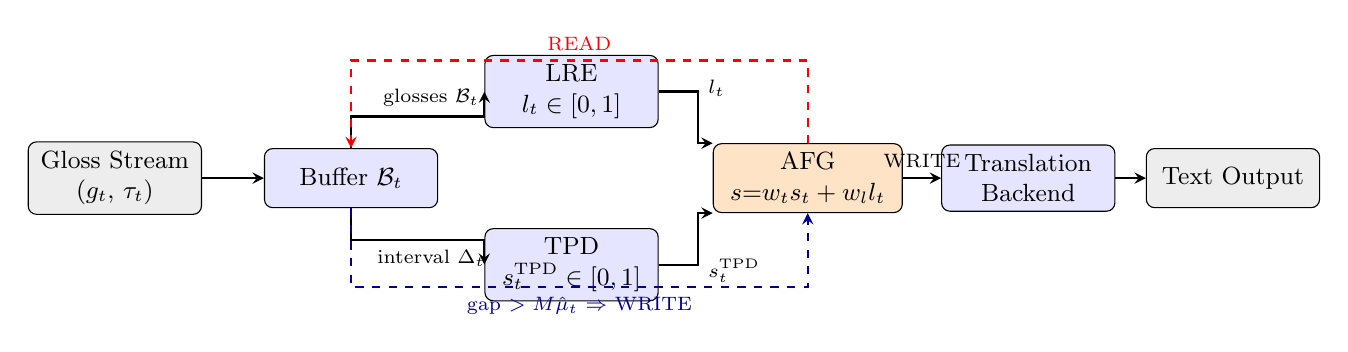
\begin{tikzpicture}[
    box/.style={rectangle, draw, rounded corners=3pt, minimum width=2.2cm, minimum height=0.75cm, align=center, fill=blue!10, font=\small},
    gatebox/.style={rectangle, draw, rounded corners=3pt, minimum width=2.4cm, minimum height=0.75cm, align=center, fill=orange!22, font=\small},
    iobox/.style={rectangle, draw, rounded corners=3pt, minimum width=2.2cm, minimum height=0.75cm, align=center, fill=gray!14, font=\small},
    arr/.style={->, thick, >=stealth},
    lbl/.style={font=\scriptsize},
]
% Nodes
\node[iobox]   (stream)  at (0, 0)    {Gloss Stream\\$(g_t,\, \tau_t)$};
\node[box]     (buffer)  at (3.0, 0)  {Buffer $\mathcal{B}_t$};
\node[box]     (lre)     at (5.8, 1.1){LRE\\$l_t \in [0,1]$};
\node[box]     (tpd)     at (5.8,-1.1){TPD\\$s_t^{\text{TPD}} \in [0,1]$};
\node[gatebox] (afg)     at (8.8, 0)  {AFG\\$s{=}w_t s_t + w_l l_t$};
\node[box]     (backend) at (11.6, 0) {Translation\\Backend};
\node[iobox]   (out)     at (14.2, 0) {Text Output};
% Connections
\draw[arr] (stream) -- (buffer);
\draw[arr] (buffer.north) -- ++(0,0.4) -| node[above, lbl, pos=0.3]{glosses $\mathcal{B}_t$} (lre.west);
\draw[arr] (buffer.south) -- ++(0,-0.4) -| node[below, lbl, pos=0.3]{interval $\Delta_t$} (tpd.west);
\draw[arr] (lre.east)  -- ++(0.5,0) |- node[above right, lbl, pos=0.15]{$l_t$} (afg.north west);
\draw[arr] (tpd.east)  -- ++(0.5,0) |- node[below right, lbl, pos=0.15]{$s_t^{\text{TPD}}$} (afg.south west);
\draw[arr] (afg) -- node[above, lbl]{WRITE} (backend);
\draw[arr] (backend) -- (out);
% READ loop (dashed red, above the diagram)
\draw[arr, dashed, red] (afg.north) -- ++(0,1.05) -| node[above, lbl, red, pos=0.25]{READ} (buffer.north);
% Proactive timeout annotation (below)
\draw[arr, dashed, blue!60!black] (buffer.south) -- ++(0,-1.0) -|
    node[below, lbl, blue!60!black, pos=0.25]{gap $> M\hat{\mu}_t$ $\Rightarrow$ WRITE} (afg.south);
\end{tikzpicture}
\caption{TLAS architecture. Each gloss $(g_t, \tau_t)$ is appended to the buffer $\mathcal{B}_t$. The Linguistic Readiness Estimator (LRE) encodes the accumulated glosses with a frozen T5 encoder and maps the pooled representation to a completeness score $l_t$; the Temporal Pause Detector (TPD) maps the inter-gloss interval $\Delta_t$ to a pause score $s_t^{\text{TPD}}$. The Adaptive Fusion Gate (AFG) combines both signals and issues WRITE (flushing the buffer to the translation backend) or READ (dashed red, continuing accumulation). A proactive timeout (dashed blue) issues WRITE directly when the elapsed gap since the last gloss exceeds $M \cdot \hat{\mu}_t$, before the next gloss arrives.}
\label{fig:tlas}
\end{figure*}

\section{Experimental Setup}

\subsection{Datasets}

\textbf{ASLG-PC12} \cite{othman2012english} is a parallel corpus of approximately 87,000 American Sign Language gloss sequences paired with English text, drawn from European Parliament proceedings converted to ASL gloss notation. Samples with fewer than three glosses or three English tokens are removed. We use a shuffled split of 50,000 training pairs, 10,000 validation pairs, and 10,000 test pairs (seed 42); sentence-level evaluation (E1) draws 100 test examples. Glosses are uppercased and English text is lowercased throughout.

\textbf{Synthetic Discourse Dataset} (contributed in this work) addresses the absence of publicly available continuous-stream ASL corpora with per-gloss timestamps. We generated 1,400 multi-sentence discourse groups using a Gemini LLM, constrained so that at least 80\% of gloss roots appear in the ASLG-PC12 or SIGNUM vocabularies. Groups span three discourse types: monologue ($\approx$40\%), deaf-deaf dialog ($\approx$30\%), and deaf-hearing dialog ($\approx$30\%). Deaf turns carry both gloss sequences and English reference translations; hearing turns carry English text only and contribute discourse context without providing gloss targets. Per-gloss arrival timestamps were generated by the same LLM with rule-based validation, calibrated to real ASL timing distributions: 300--650~ms per sign within a sentence and 1.5--7~s between sentences. The first 200 groups (888 deaf sentences) constitute the test split used in E2; the remaining 1,200 groups ($\approx$5,234 context pairs) form the training split.

\textbf{SIGNUM} consists of 779 German Sign Language sentence pairs drawn from everyday conversational topics. We include these during T5 fine-tuning to expose the model to a distinct sign language vocabulary and domain; a held-out subset is also used for cross-dataset generalization evaluation.

\textbf{Stream files} provide three manually timestamped gloss streams for qualitative E3 evaluation: \texttt{monologue1} (108 tokens, 20 sentences), \texttt{monologue2} ($\approx$80 tokens, 14 sentences), and \texttt{dialog3} ($\approx$150 tokens, $\approx$30 sentences across two speakers). Inter-sentence gaps range from 2 to 7~s, matching the synthetic dataset's timing distribution.

\subsection{Evaluation Paradigms}

We evaluate under three complementary paradigms.

\textbf{E1 — Sentence-level evaluation} uses 100 ASLG-PC12 test sentences with synthetic uniform timestamps (450~ms per gloss). All policies operate within known sentence boundaries and receive identical input; the temporal signal is therefore neutralized ($s_t^{\text{TPD}} \approx 0$) and TLAS degenerates to max-lag triggering. E1 measures pure linguistic translation quality and provides a controlled comparison between TLAS-linguistic and LSG.

\textbf{E2 — Continuous-stream discourse evaluation} is the primary experiment. Each of the 200 test discourse groups is fed as a single unbroken gloss stream using the LLM-generated per-gloss timestamps; policies receive no oracle sentence boundaries. Inter-sentence pauses of 1.5--7~s provide a strong temporal signal that TLAS exploits via the proactive timeout, while baselines fragment the stream arbitrarily. We report corpus-level BLEU for the full test set and break results down by discourse position to measure how quality evolves within a group.

\textbf{E3 — Real stream file evaluation} is a qualitative demonstration on the three manually timestamped stream files. We inspect produced segments, boundary recall relative to ground-truth sentence count, and representative translation examples.

\subsection{Evaluation Metrics}

We report four complementary metrics. \textbf{BLEU} \cite{papineni2002bleu} measures corpus-level n-gram precision with a brevity penalty, computed with SacreBLEU for reproducibility. \textbf{ROUGE-L} \cite{lin2004rouge} measures longest common subsequence overlap, capturing sentence-level recall. \textbf{SBERT cosine similarity} encodes each hypothesis and reference with Sentence-BERT and computes their cosine similarity, providing a semantic fluency signal robust to paraphrase. \textbf{chrF++} computes character n-gram F-score with word unigram recall, which is informative for morphologically varied outputs.

For E2, we additionally report the \textbf{retention rate} (policy BLEU divided by oracle BLEU) and \textbf{position-stratified BLEU} (corpus BLEU computed separately per discourse position), which reveals whether policies maintain translation quality throughout a discourse group or degrade at later positions due to accumulated segmentation error.

\subsection{Hyperparameters}

Table~\ref{tab:hyperparams} summarizes all TLAS hyperparameters. The TPD smoothing factor $\alpha$ and pause multiplier $M$ were set from the inter-gloss timing statistics of the training data; the AFG weights and thresholds were validated on 20 held-out discourse groups not included in the test split.

\begin{table}[t]
\centering
\caption{TLAS hyperparameter settings.}
\label{tab:hyperparams}
\begin{tabular}{lll}
\toprule
\textbf{Component} & \textbf{Parameter} & \textbf{Value} \\
\midrule
\multirow{3}{*}{TPD} & EMA smoothing $\alpha$ & 0.3 \\
                     & Pause multiplier $M$ & 2.5 \\
                     & EMA prior $\hat{\mu}_0$ & 450~ms \\
\midrule
\multirow{2}{*}{LRE} & Hidden dim & 256 \\
                     & Dropout & 0.1 \\
\midrule
\multirow{6}{*}{AFG} & $w_t$ (temporal weight) & 0.4 \\
                     & $w_l$ (linguistic weight) & 0.6 \\
                     & Joint threshold $\theta$ & 0.40 \\
                     & Strong pause threshold & 0.80 \\
                     & Min.\ readiness for pause & 0.30 \\
                     & Max lag $L_{\max}$ & 6 \\
\midrule
\multirow{2}{*}{Policy} & Discourse context window & 3 \\
                        & Wait-k lag $k$ & 3 \\
\bottomrule
\end{tabular}
\end{table}


\section{Results}

\subsection{E2: Continuous-Stream Discourse Evaluation}

E2 is the primary experiment. Table~\ref{tab:e2_t5} presents T5 results on 200 discourse groups (888 sentences). Two distinct performance tiers are immediately apparent. The three TLAS variants cluster between 17 and 24 BLEU (70--97\% retention), while all three baselines fall below 7 BLEU (under 20\% retention). This separation holds across every metric — ROUGE-L, SBERT cosine similarity, and chrF++ — confirming that the gap is not an artifact of the BLEU brevity penalty.

\begin{table}[t]
\centering
\caption{E2 continuous-stream results, T5 backend (200 groups, 888 sentences). Ret.\ = BLEU / oracle BLEU. Best streaming value in \textbf{bold}.}
\label{tab:e2_t5}
\small
\begin{tabular}{lccc}
\toprule
\textbf{Policy} & \textbf{BLEU} & \textbf{ROUGE-L} & \textbf{Ret.} \\
\midrule
Batch (oracle) $\uparrow$ & 24.49 & .593 & --- \\
\midrule
Batch             &  1.74 & .068 &  7.1\% \\
Wait-k ($k$=3)    &  1.86 & .286 &  7.6\% \\
TransLLaMa        &  4.76 & .385 & 19.4\% \\
\midrule
LSG               &  6.43 & .398 & 26.3\% \\
TLAS-linguistic   & 17.18 & .474 & 70.1\% \\
TLAS-temporal     & \textbf{23.70} & \textbf{.564} & \textbf{96.8\%} \\
TLAS              & 21.51 & .536 & 87.9\% \\
\bottomrule
\end{tabular}
\end{table}

TLAS-temporal achieves 96.8\% retention, recovering nearly all of the oracle's translation quality through temporal segmentation alone. The trained LRE provides a meaningful additional contribution: TLAS-linguistic achieves 70.1\% retention compared to LSG's 26.3\%, a 2.7$\times$ improvement that directly measures the benefit of learned readiness estimation over heuristic KL-divergence scoring. The full TLAS (87.9\%) falls between the two ablations in E2 because the linguistic signal, while helpful, introduces occasional conservative delays that the proactive timeout cannot compensate for when the LRE is uncertain.

Table~\ref{tab:e2_backends} extends the comparison to all three backends. The superiority of TLAS-temporal and full TLAS replicates across all three backends: both achieve retention above 80\% on T5 and Gemini and above 81\% and 92\% on Ollama, respectively, against traditional baselines that peak at 57\% on the most generous backend. TLAS-linguistic shows more backend-dependent behavior: it leads on T5 (70.1\%) and Gemini (64.7\%) but falls behind LSG on Ollama (60.1\% vs.\ 68.6\%), a reversal attributed to the LRE head being trained on T5 encoder representations and less well-calibrated for the weaker Ollama decoder's output characteristics.

\begin{table*}[t]
\centering
\caption{E2 results across all three backends. Ret.\ = BLEU / backend oracle BLEU.}
\label{tab:e2_backends}
\small
\begin{tabular}{lcccccc}
\toprule
& \multicolumn{2}{c}{\textbf{T5} (oracle: 24.49)} & \multicolumn{2}{c}{\textbf{Gemini} (oracle: 24.39)} & \multicolumn{2}{c}{\textbf{Ollama} (oracle: 12.53)} \\
\cmidrule(lr){2-3}\cmidrule(lr){4-5}\cmidrule(lr){6-7}
\textbf{Policy} & BLEU & Ret. & BLEU & Ret. & BLEU & Ret. \\
\midrule
Batch           &  1.74 &  7.1\% &  5.71 & 23.4\% &  1.90 & 15.2\% \\
Wait-k          &  1.86 &  7.6\% & 11.49 & 47.1\% &  7.12 & 56.8\% \\
TransLLaMa      &  4.76 & 19.4\% & 12.54 & 51.4\% &  5.64 & 45.0\% \\
\midrule
LSG             &  6.43 & 26.3\% & 14.88 & 61.0\% &  8.59 & 68.6\% \\
TLAS-linguistic & 17.18 & 70.1\% & 15.79 & 64.7\% &  7.53 & 60.1\% \\
TLAS-temporal   & \textbf{23.70} & \textbf{96.8\%} & \textbf{22.13} & \textbf{90.7\%} & \textbf{11.56} & \textbf{92.3\%} \\
TLAS            & 21.51 & 87.9\% & 21.46 & 88.0\% & 10.23 & 81.6\% \\
\bottomrule
\end{tabular}
\end{table*}

The Gemini and Ollama traditional baselines achieve higher absolute retention than T5 baselines because the larger LLMs are more capable of completing incoherent gloss fragments into plausible English text, partially masking the segmentation failure. Despite this, TLAS-temporal and full TLAS lead every traditional baseline (Batch, Wait-k, TransLLaMa) by at least 24 percentage points on every backend.

Table~\ref{tab:position} reports BLEU stratified by sentence position within the discourse group (T5 backend). Baseline policies produce near-zero BLEU by position 2 or 3: Batch (non-oracle) collapses because the long-string translation only aligns with the first sentence, and Wait-k degrades monotonically as earlier cross-boundary errors shift alignment. The three TLAS variants maintain stable BLEU at all positions, with TLAS-temporal staying within 5 BLEU points of the oracle at every depth.

\begin{table*}[t]
\centering
\caption{Position-stratified BLEU in E2 (T5 backend). Position 0 = first sentence in group; 4+ = fifth or later.}
\label{tab:position}
\small
\begin{tabular}{lccccc}
\toprule
\textbf{Policy} & \textbf{Pos 0} & \textbf{Pos 1} & \textbf{Pos 2} & \textbf{Pos 3} & \textbf{Pos 4+} \\
\midrule
Batch (oracle) $\uparrow$ & 18.73 & 29.31 & 23.20 & 27.44 & 23.41 \\
\midrule
Batch          &  6.77 &  2.14 &  0.28 &  0.01 &  0.00 \\
Wait-k         &  4.68 &  2.03 &  1.83 &  0.84 &  0.27 \\
TransLLaMa     &  7.17 &  6.27 &  3.78 &  4.44 &  1.39 \\
\midrule
LSG            & 11.69 &  7.58 &  5.31 &  4.43 &  1.84 \\
TLAS-linguistic& 17.68 & 18.56 & 15.32 & 20.63 & 18.68 \\
TLAS-temporal  & \textbf{20.10} & \textbf{25.52} & \textbf{21.67} & \textbf{27.03} & \textbf{21.28} \\
TLAS           & 19.57 & 21.35 & 19.20 & 25.53 & 20.20 \\
\bottomrule
\end{tabular}
\end{table*}

\subsection{E1: Sentence-Level Evaluation}

Table~\ref{tab:e1} presents sentence-level results on 100 ASLG-PC12 test examples with synthetic uniform timestamps. Because all policies receive isolated sentences with no inter-sentence pauses, the TPD emits near-zero scores throughout and TLAS degenerates to max-lag ($L_{\max}=6$) triggering. Under these conditions TLAS-temporal (79.7\% retention) and full TLAS (76.3\%) lead all streaming methods, demonstrating that the max-lag safety valve provides adequate within-sentence segmentation quality even when the temporal cue is suppressed. LSG collapses to near-zero BLEU (0.01) because the KL-divergence threshold fires too aggressively on short T5 encoder prefixes, immediately committing to translations with fewer than two glosses buffered; TLAS-linguistic (61.0\%) substantially avoids this failure by using the calibrated LRE readiness score instead.

\begin{table}[t]
\centering
\caption{E1 sentence-level results, T5 backend ($n$=100, synthetic timestamps).}
\label{tab:e1}
\small
\begin{tabular}{lccc}
\toprule
\textbf{Policy} & \textbf{BLEU} & \textbf{ROUGE-L} & \textbf{Ret.} \\
\midrule
Batch $\uparrow$  & 73.84 & .919 & --- \\
\midrule
TLAS-temporal     & 58.88 & .869 & 79.7\% \\
TLAS              & 56.36 & .867 & 76.3\% \\
TLAS-linguistic   & 45.04 & .824 & 61.0\% \\
TransLLaMa        & 43.35 & .821 & 58.7\% \\
Wait-k ($k$=3)    & 31.84 & .757 & 43.1\% \\
LSG               &  0.01 & .149 & $\approx$0\% \\
\bottomrule
\end{tabular}
\end{table}

The ranking of TLAS-linguistic (61.0\%) above TransLLaMa (58.7\%) in E1, combined with TLAS-linguistic's 2.7$\times$ BLEU advantage over LSG in E2, consistently supports the benefit of the trained LRE head across both evaluation settings.

\subsection{Timestamp Robustness}

Table~\ref{tab:robustness} reports BLEU under three timestamp conditions for TLAS variants on the E2 test set (T5 backend). TLAS-linguistic varies by less than 0.1 BLEU points across all three conditions, confirming zero sensitivity to timestamp quality and pure reliance on the LRE signal and max-lag fallback. TLAS-temporal degrades by 57\% from realistic to noisy (23.70 $\to$ 10.07): Gaussian jitter of $\sigma=500$~ms corrupts the EMA, causing premature or delayed proactive timeouts. A crossing point occurs at uniform timestamps: TLAS-linguistic (17.09) overtakes TLAS-temporal (15.61), because uniform gaps suppress the temporal signal to exactly zero while the LRE continues to operate normally. Full TLAS degrades gracefully (21.51 $\to$ 11.53) relative to temporal-only because the LRE provides a stabilizing floor; the remaining 46\% decline reflects the temporal weight ($w_t=0.4$) pulling the combined score toward corrupted TPD outputs.

\begin{table}[t]
\centering
\caption{Timestamp robustness: BLEU under three conditions (T5, E2). Oracle ceiling: 24.49 BLEU.}
\label{tab:robustness}
\small
\begin{tabular}{lccc}
\toprule
\textbf{Policy} & \textbf{Realistic} & \textbf{Uniform} & \textbf{Noisy} \\
\midrule
TLAS-temporal   & \textbf{23.70} & 15.61 & 10.07 \\
TLAS            & 21.51 & 16.68 & 11.53 \\
TLAS-linguistic & 17.18 & \textbf{17.09} & \textbf{17.18} \\
\bottomrule
\end{tabular}
\end{table}

\subsection{Cross-Dataset Generalization and Context Benefit}

On the SIGNUM German Sign Language dataset (779 pairs, completely out-of-domain from T5's ASLG-PC12 training data), TLAS achieves 3.47 BLEU against a batch oracle of 3.51 BLEU, a retention rate of 99.1\%. The low absolute scores reflect domain shift rather than policy failure; the near-complete retention confirms that TLAS's segmentation behavior generalizes across sign language vocabularies without retraining.

To isolate the contribution of the discourse context window, we evaluated TLAS without context (context\_window=0) versus the default (context\_window=3) on 200 E2 groups. Context raises BLEU from 2.98 to 5.02, a 68\% relative improvement, indicating that prior translations provide genuinely useful disambiguation even in the streaming setting where each segment is translated independently.

\section{Discussion}

\subsection{The Two-Tier Separation in Continuous Stream Evaluation}

The E2 results establish a clear two-tier structure across all four metrics: TLAS variants (TLAS-temporal, TLAS, TLAS-linguistic) achieve 17--24 BLEU, while all baselines cluster between 1 and 15 BLEU, with Wait-k at 1.86 (7.6\% retention) and Batch (non-oracle) at 1.74 (7.1\% retention). This separation is consistent across BLEU, ROUGE-L, SBERT, and chrF++, confirming it is not an artifact of metric choice. The position-stratified analysis (Table~\ref{tab:position}) reveals the mechanism: Wait-k collapses from 4.68 BLEU at discourse position 0 to 0.27 at position 4+, and Batch (non-oracle) reaches 0.00 BLEU by position 4+. TLAS-temporal, by contrast, sustains 20.10--27.03 BLEU across all five position bins, tracking the oracle trajectory (18.73--29.31 BLEU). The root cause is boundary detection, not translation capability per se. Baselines that fragment across sentence boundaries submit incoherent gloss subsets to the translator, which produces outputs with near-zero overlap with any individual reference sentence. TLAS's proactive timeout, firing at inter-sentence gaps of 2--7 seconds, aligns each output segment with a true sentence boundary, presenting the translator with coherent inputs regardless of discourse depth.

\subsection{Temporal Signal Is the Primary Segmentation Mechanism}

Under realistic timestamps (E2, T5 backend), TLAS-temporal achieves 96.8\% retention, within 3.2 percentage points of the oracle ceiling, demonstrating that the TPD pause signal alone is sufficient for near-perfect segmentation. TLAS-linguistic, which receives no temporal information, retains 70.1\%, a 26.7-point retention gap. The difference is entirely attributable to segmentation fidelity rather than translation quality, since both ablations use the same T5 translator. The EMA $\hat{\mu}_t$ tracks within-sentence timing (300--650~ms per sign) and cleanly detects inter-sentence pauses (2--7~s) via the proactive timeout, which fires before the next gloss arrives rather than waiting for a gloss event to trigger the reactive AFG pipeline. TLAS-linguistic, lacking this signal, relies on the LRE readiness score and the max\_lag=$6$ safety valve; this produces segments that occasionally span boundaries or subdivide sentences, explaining the systematic BLEU loss at later discourse positions (Table~\ref{tab:position}).

The full TLAS fusion ($w_t=0.4$, $w_l=0.6$) achieves 87.9\% retention, below TLAS-temporal but above TLAS-linguistic. The AFG's strong-pause override ($s_{\mathrm{TPD}} \geq 0.8$) ensures that unambiguous temporal boundaries are respected even when the LRE score is low, while the joint threshold ($s \geq 0.40$) allows the LRE to trigger early translation for linguistically complete prefixes, reducing average lag within sentences. The fusion therefore does not simply average the two signals: it uses temporal evidence for hard boundary detection and linguistic evidence to accelerate translation when temporal cues are weak.

\subsection{Evaluation Paradigm: E1 Cannot Assess Streaming Segmentation}

In E1 (sentence-level, uniform synthetic timestamps), the TPD receives inter-gloss gaps of exactly 450~ms throughout, producing pause\_score $\approx 0$ at every step. TLAS therefore degenerates to its max\_lag safety valve, firing every 6 glosses and behaving as a fixed-window policy regardless of sentence length. E1 evaluates each sentence in isolation (oracle boundaries are implicit in the single-sentence structure), so no policy can fail on cross-boundary detection. Table~\ref{tab:e1} reflects this: Wait-k achieves 43.1\% retention on E1 (T5) but only 7.6\% on E2, and TransLLaMa achieves 58.7\% on E1 but only 19.4\% on E2. These collapses do not appear in E1 because there are no cross-sentence boundaries to fragment across. Prior streaming translation benchmarks operate exclusively in E1-like settings, which cannot detect this failure mode.

Our E2 paradigm corrects this by removing oracle segmentation, replacing synthetic uniform timing with LLM-generated per-gloss timestamps (300--650~ms intra-sentence, 1500--7000~ms inter-sentence), and measuring whether each policy can reconstruct sentence structure from the raw gloss-and-timestamp stream. Under E2, TLAS-temporal's retention advantage over Wait-k grows from 36.6 percentage points (E1: 79.7\% vs.\ 43.1\%) to 89.2 percentage points (E2: 96.8\% vs.\ 7.6\%), a three-fold amplification that E1 conceals entirely. We argue that any streaming policy intended for deployment in a continuous signing context must be evaluated in an E2-like setting; an E1-only evaluation cannot assess the core challenge of real-time sentence boundary detection.

\subsection{Trained Readiness Outperforms Heuristic Estimation}

The LSG-to-TLAS-linguistic progression isolates, approximately, the contribution of the trained LRE head over the KL-divergence heuristic, though we note that the two systems differ in two respects: the readiness estimator (trained vs.\ heuristic) and the discourse context window (context\_window=3 for TLAS-linguistic vs.\ context\_window=0 for LSG). In E1 (T5 backend, Table~\ref{tab:e1}), LSG collapses to near-zero BLEU (0.01) because the KL-divergence threshold fires immediately on short T5 encoder prefixes, while TLAS-linguistic achieves 45.04 BLEU (61.0\% retention). On the Gemini backend, where the KL heuristic does not catastrophically fail, the E1 gap is smaller: LSG achieves 15.11 BLEU and TLAS-linguistic achieves 16.99 BLEU, a 12.4\% relative improvement. In E2 (Table~\ref{tab:e2_t5}), the gap is large across all backends: on T5, LSG reaches 6.43 BLEU (26.3\% retention) while TLAS-linguistic reaches 17.18 BLEU (70.1\% retention), a 167\% relative improvement. The E2 gap reflects a compounding effect: the KL-divergence heuristic produces noisier WRITE decisions, leading to fragmented segments whose alignment errors accumulate across the discourse group. The trained LRE, supervised on ROUGE-L oracle labels with monotonicity enforcement, produces calibrated readiness scores that correctly defer translation for short or syntactically incomplete prefixes while triggering it for linguistically complete ones.

\subsection{Timestamp Robustness and Deployment Considerations}

The robustness experiments (Table~\ref{tab:robustness}) reveal that the temporal and linguistic signals are complementary across a range of timing conditions. TLAS-temporal achieves the highest BLEU under realistic timestamps (23.70 BLEU, 96.8\% retention) but degrades by 57\% under Gaussian jitter ($\sigma=500$~ms), reaching 10.07 BLEU, because EMA corruption causes premature or delayed proactive timeouts. TLAS-linguistic, by contrast, varies by less than 0.1 BLEU points across all three conditions, constituting a timestamp-invariant floor. A crossing point occurs at uniform timestamps (as arise from fixed-rate video frame delivery): TLAS-linguistic (17.09) overtakes TLAS-temporal (15.61) because uniform gaps suppress the temporal signal to zero while the LRE continues to operate normally. The full TLAS fusion degrades more gracefully than temporal-only (11.53 vs.\ 10.07 under noisy timestamps), since the linguistic weight ($w_l=0.6$) provides a stabilizing floor; however, a 46\% decline from realistic to noisy conditions confirms that the temporal component remains the dominant vulnerability when timestamp quality is poor.

These results carry direct implications for deployment. In systems with reliable sub-100~ms timestamp precision (purpose-built sign recognition pipelines), TLAS-temporal maximizes quality. In systems with known timing variance (video codecs, high-latency GPU inference), TLAS-linguistic provides a robust fallback. The full TLAS fusion is recommended as the default for systems where timestamp reliability is unknown or variable, as it outperforms linguistic-only under reliable timing and outperforms temporal-only under noise.

\subsection{Limitations}

Three limitations bound the current study. First, the E2 discourse dataset is synthetically generated by a large language model under vocabulary constraints; while per-gloss timestamps are validated against empirical signing rates (300--650~ms intra-sentence, 1500--7000~ms inter-sentence), the conversation topics and turn structures may not fully represent authentic Deaf community interactions. Second, the translation pipeline evaluated here begins at the gloss level: the end-to-end system from raw video to text has not been integrated, and recognition errors from the vision module would interact with the TPD and LRE in ways not measured here. Third, Average Lagging and LAAL are computed over simulated streams; wall-clock inference latency under real-time constraints, where GPU memory bandwidth, tokenizer overhead, and API round-trip times all compound, has not been measured.

\section{Conclusion}

We presented TLAS (Temporal-Linguistic Adaptive Streaming), a streaming translation policy that integrates temporal pause detection and learned linguistic readiness as complementary signals for continuous sign language segmentation and translation. The TPD tracks the exponential moving average $\hat{\mu}_t$ of inter-gloss intervals to detect inter-sentence pauses; the LRE applies a trained head on frozen T5 encoder states to estimate whether accumulated glosses form a translatable unit; and the AFG fuses both signals into WRITE decisions via a weighted threshold gate with a strong-pause override. A proactive timeout mechanism fires before the next gloss arrives whenever the inter-gloss gap exceeds $M \cdot \hat{\mu}_t$, enabling clean sentence segmentation during natural signing pauses without requiring a subsequent gloss event.

On the primary E2 continuous-stream evaluation (200 discourse groups, 888 sentences), TLAS-temporal achieves 96.8\% retention of oracle quality (23.70 vs.\ 24.49 BLEU, T5 backend) and the full TLAS fusion achieves 87.9\%, while Wait-k reaches only 7.6\% and Batch (non-oracle) only 7.1\%. Position-stratified BLEU confirms that TLAS sustains near-uniform quality across all discourse positions (20.10--27.03 BLEU for TLAS-temporal), whereas baselines collapse by position 2 due to cross-boundary fragmentation. The trained LRE head outperforms the KL-divergence heuristic (LSG) by 12.4\% relative in E1 and 167\% relative in E2. Timestamp robustness analysis shows the signals are complementary: TLAS-temporal maximizes performance under reliable timing (96.8\% retention) while TLAS-linguistic provides a stable 70.1\% retention floor invariant to timestamp noise. On the SIGNUM out-of-domain evaluation, TLAS achieves 99.1\% retention of the batch oracle, demonstrating strong cross-lingual generalization without retraining.

Two directions represent the most consequential extensions of this work. First, replacing the T5 decoder with a state-space model (Mamba) would reduce per-step inference from $O(n^2)$ to $O(1)$, eliminating the need to re-encode the full buffer at each step and enabling the hidden state to propagate discourse context across sentence boundaries implicitly, without a sliding context window. Second, optimizing the AFG fusion weights and thresholds via reinforcement learning, treating the quality-latency trade-off as a learnable reward signal, would replace manually tuned hyperparameters with a policy adapted directly to the target deployment environment.

\bibliographystyle{IEEEtran}
\bibliography{references}

\end{document}

